\documentclass[11pt, a4paper]{article}

% Basic packages
\usepackage{amsmath,amssymb,amsfonts}
\usepackage{bm,ltablex,microtype}
\usepackage{graphicx}
\usepackage[utf8]{inputenc}
\usepackage{parskip}
\usepackage[section]{placeins}
\usepackage[capitalise, noabbrev]{cleveref}
\usepackage{fancyvrb}
\usepackage{csvsimple}
\usepackage{booktabs}
\usepackage{multicol}
\usepackage[margin=3cm]{geometry}
\usepackage[table,xcdraw]{xcolor}
\usepackage{tikz}
\usetikzlibrary{math,calc,positioning}

\usepackage{todonotes}

% Set up fonts
% \usepackage{fontspec}
% \usepackage{unicode-math}
% \setmainfont{STIX Two Text}
% \setmathfont{STIX Two Math}

\title{FYS-STK4155 - Project1}
\author{Gard, Are, David Andreas Bordvik}
\date{\today}

\begin{document}

\maketitle
  
\section*{Motivation}
In Project 1, we are tasked to study various regressions methods, such as Ordinary Least Squares, Ridge and Lasso. Our first area of study is how to fit polynomials to a specific two-dimensional function called Franke's Function. Our motivation behind fitting polynomials to Frank's function is to test the implementation of our regression algorithms, as well as studying various techniques such as bootstrapping and measurements such as the bias-variance tradeoff. Finally, we will move on to use real digital terrain data for our analysis.

Frank's function is given on the form

\begin{align*}
  f(x,y) &= \frac{3}{4}\exp{\left(-\frac{(9x-2)^2}{4} - \frac{(9y-2)^2}{4}\right)}+\frac{3}{4}\exp{\left(-\frac{(9x+1)^2}{49}- \frac{(9y+1)}{10}\right)} \\
  &+\frac{1}{2}\exp{\left(-\frac{(9x-7)^2}{4} - \frac{(9y-3)^2}{4}\right)} -\frac{1}{5}\exp{\left(-(9x-4)^2 - (9y-7)^2\right) }
\end{align*}

with a 3-dimensional plot given in Figure \ref{fig:1}

\begin{figure}[h]
  \centering
  \includegraphics[scale=0.75]{figures/franke_function_preview.pdf}
  \caption{\label{fig:1}Plot of the Franke Function}
\end{figure}

\section*{Theory}
MSE value between $\boldsymbol{y}$ and $\boldsymbol{\hat y}$ is defined as;
\begin{equation}
    MSE(\boldsymbol{y},\boldsymbol{\tilde{y}}) = \frac{1}{n}
    \sum_{i=0}^{n-1}(y_i-\tilde{y}_i)^2
\end{equation}

The $R^2$ value between $\boldsymbol{y}$ and $\boldsymbol{\hat y}$ is defined as;
\begin{equation}
    R^2(\boldsymbol{y}, \tilde{\boldsymbol{y}}) = 1 - \frac{\sum_{i=0}^{n - 1} (y_i - \tilde{y}_i)^2}{\sum_{i=0}^{n - 1} (y_i - \bar{y})^2}
\end{equation}

The mean value of $\boldsymbol{y}$ is defined as;
\begin{equation}
    \bar{y} =  \frac{1}{n} \sum_{i=0}^{n - 1} y_i
\end{equation}

The variance of $\boldsymbol{y}$ is defined as;
\begin{equation}
    \mathrm{var}[\boldsymbol{x}]=\frac{1}{n}\sum_{i=0}^{n-1}(x_i- \overline{x})^2=\mathbb{E}\left[(\bm{y}-\bm{\tilde{y}})^2\right]
\end{equation}

\section*{Exercise 1}





\begin{figure}
  \centering
  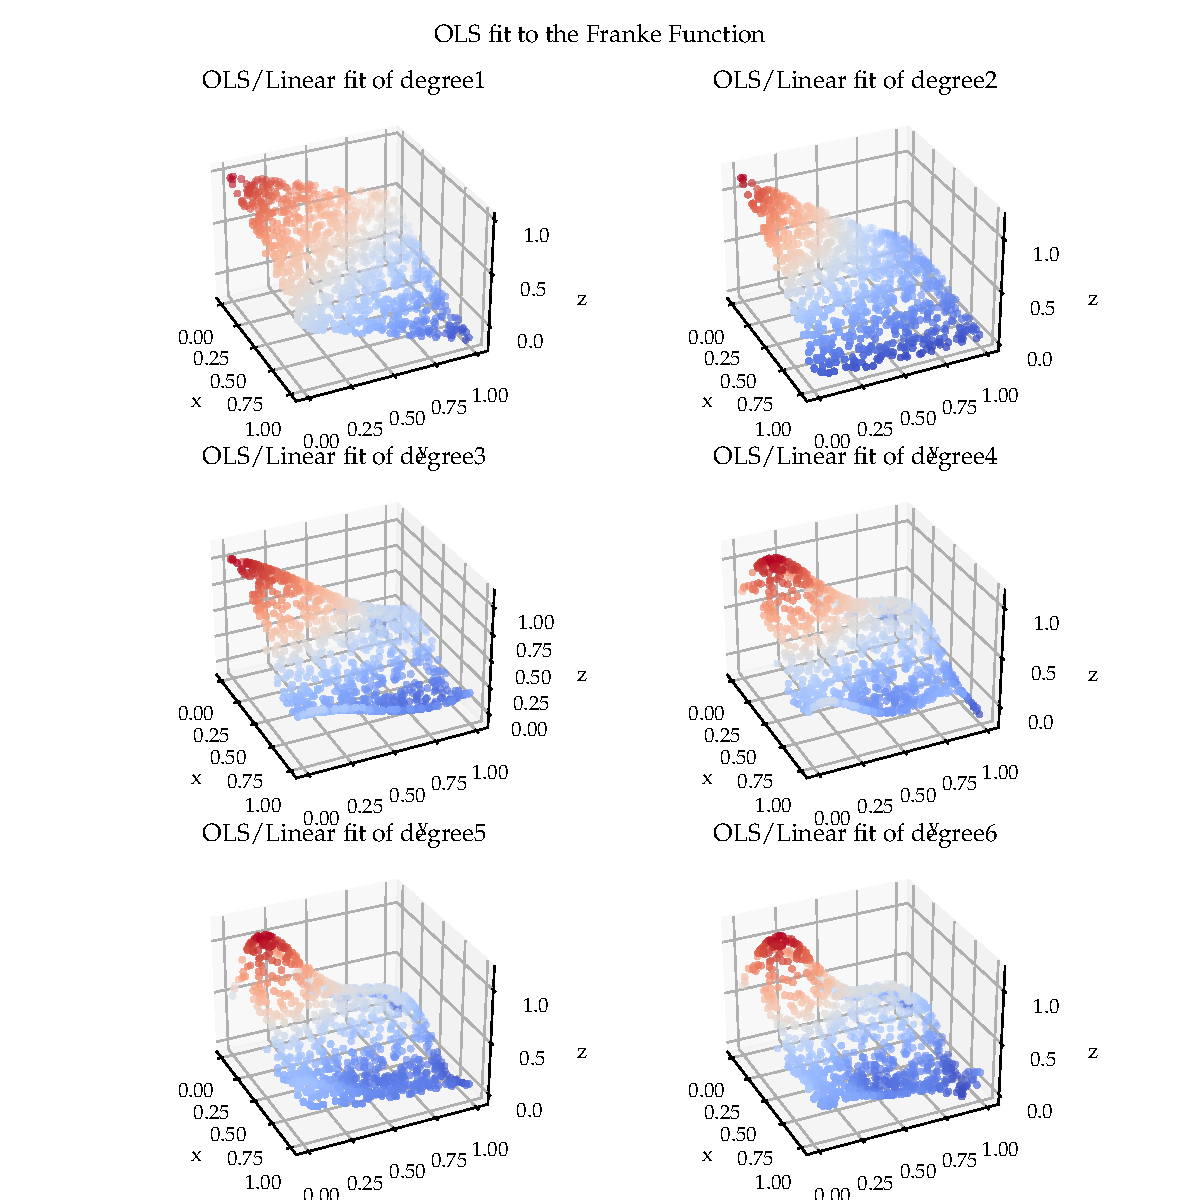
\includegraphics[scale=0.85]{figures/franke_function_OLS_fit.pdf}
  \caption{?}
  \label{fig: ?}
\end{figure}

\begin{figure}
  \centering
  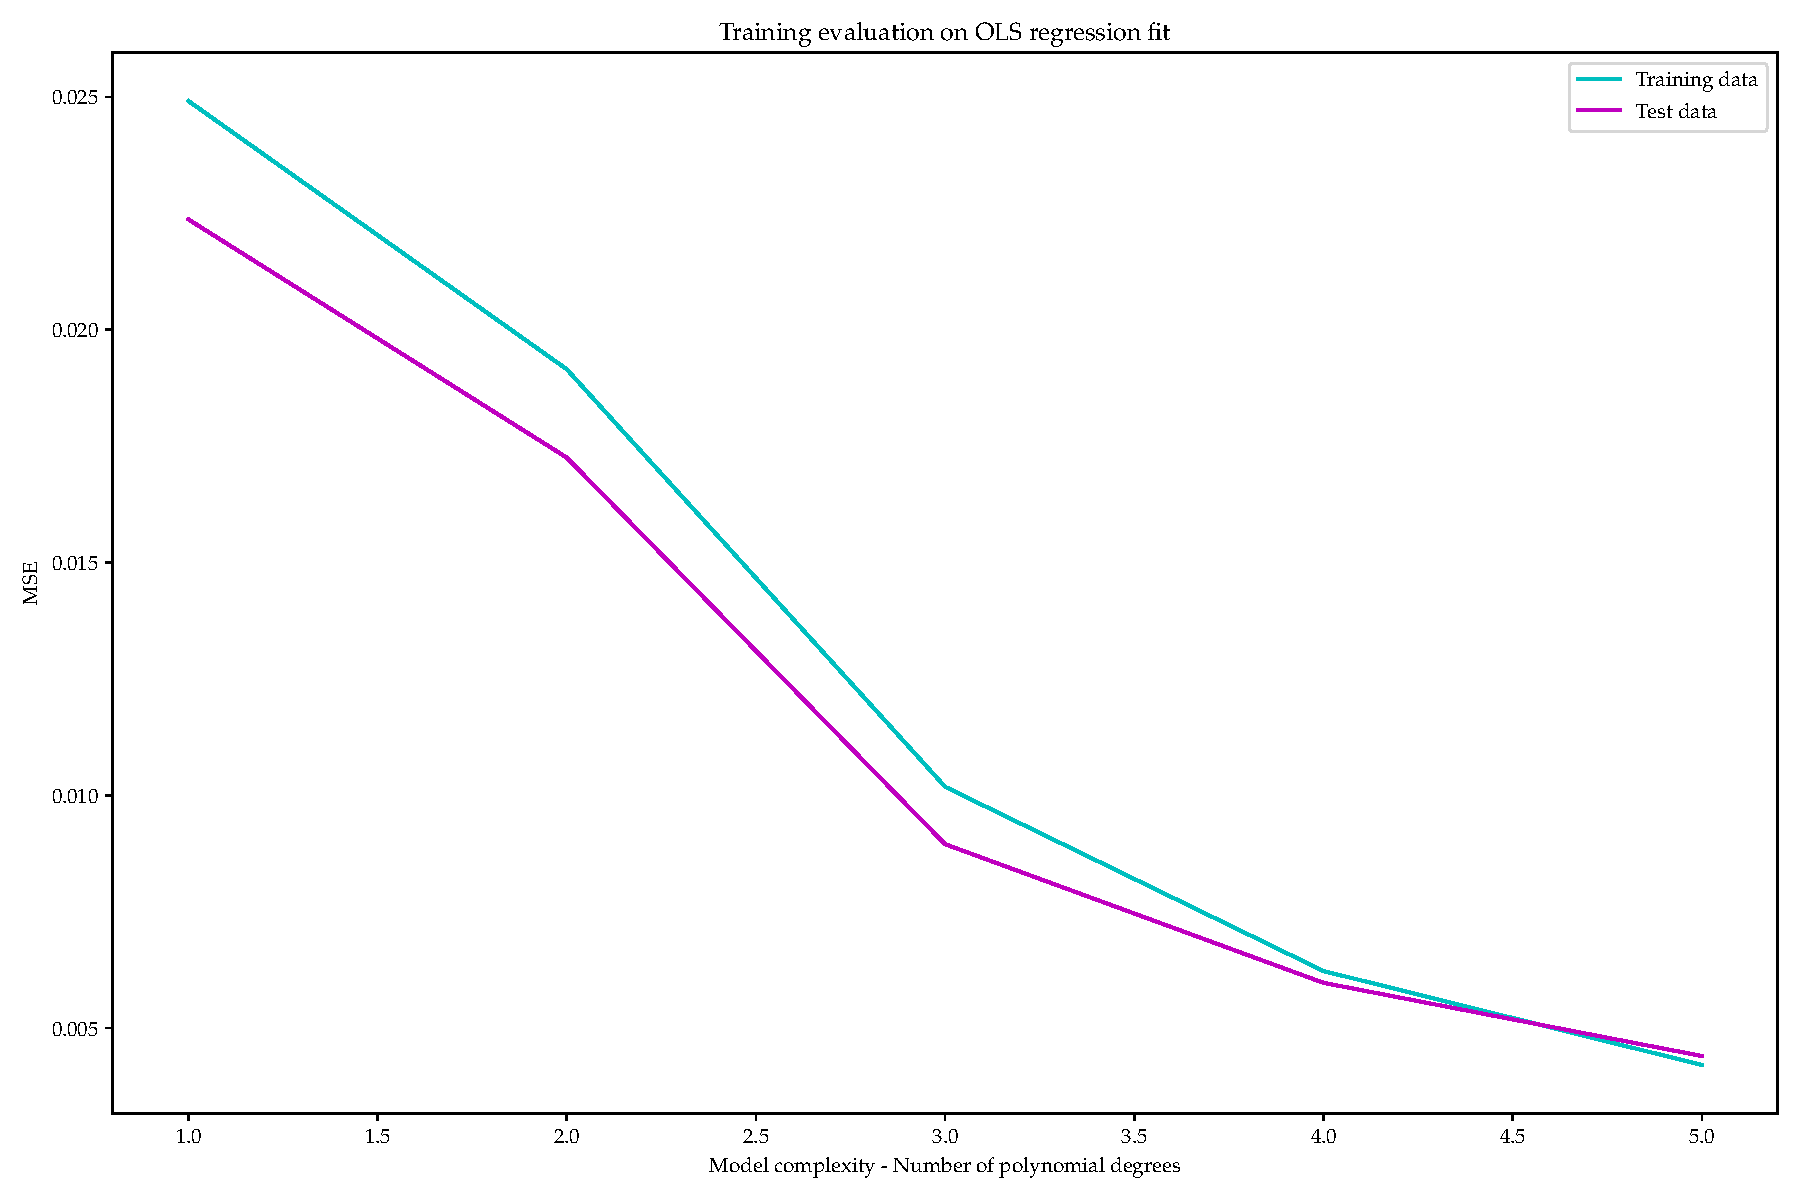
\includegraphics[scale=0.45]{figures/franke_function_OLS_evaluate_fit.pdf}
  \caption{?}
  \label{fig: ?}
\end{figure}

\begin{figure}
  \centering
  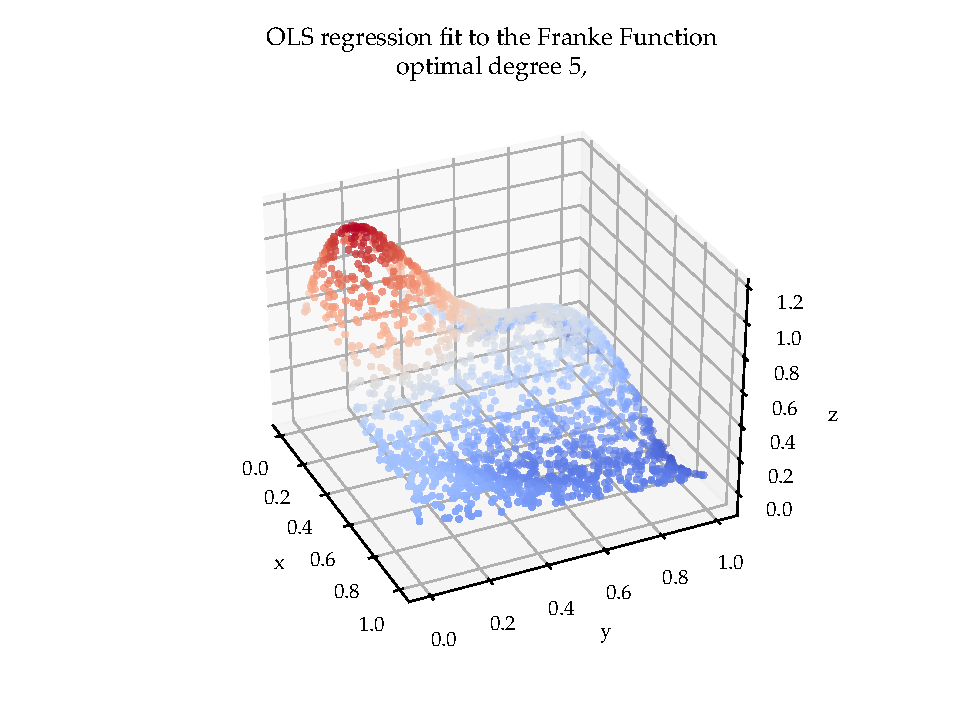
\includegraphics[scale=0.85]{figures/franke_function_OLS_best_fit.pdf}
  \caption{?}
  \label{fig: ?}
\end{figure}


\section*{Exercise 2}
Moving on to the bias-variance trade-off analysis, we start off by showing that 

\[
  C(\bm{X},\bm{\beta}) =\frac{1}{n}\sum_{i=0}^{n-1}(y_i-\tilde{y}_i)^2=\mathbb{E}\left[(\bm{y}-\bm{\tilde{y}})^2\right]
\]

Can be rewritten as

\[
\mathbb{E}\left[(\bm{y}-\bm{\tilde{y}})^2\right]=\frac{1}{n}\sum_i(f_i-\mathbb{E}\left[\bm{\tilde{y}}\right])^2+\frac{1}{n}\sum_i(\tilde{y}_i-\mathbb{E}\left[\bm{\tilde{y}}\right])^2+\sigma^2.
\]

where the terms are respectively $(\text{bias})^2$, variance and noise. For simplicity, assume that we have a dataset where the data is generated from a noisy model

\[\bm{y} = f(\bm{x}) + \bm{\epsilon}\]

Furthermore, we will assume that the residuals $\epsilon$ are independant and normally distributed $\epsilon \sim \mathcal{N}(0, \sigma^2)$. Finally, $\bm{\tilde{y}} = \bm{X}\bm{\beta}$ is our approximation to the functions $f$. Start off by adding and subtracting $\mathbb{E}\left[\bm{\tilde{y}}\right]$ inside the expectation value.

\[
  \mathbb{E}\left[(\bm{y}-\bm{\tilde{y}})^2\right] 
  = \mathbb{E}\left[(\bm{y}-\bm{\tilde{y}} + \mathbb{E}\left[\bm{\tilde{y}}\right] - \mathbb{E}\left[\bm{\tilde{y}}\right])^2\right] 
\]
\[
  = \mathbb{E}\left[((\bm{y} - \mathbb{E}\left[\bm{\tilde{y}}\right]) - (\bm{\tilde{y}} - \mathbb{E}\left[\bm{\tilde{y}}\right]))^2\right]
\]
By using the fact that $\bm{y} = f(\bm{x}) + \bm{\epsilon}$
we can rewrite this as
\[
  = \mathbb{E}\left[((f(\bm{x}) - \mathbb{E}\left[\bm{\tilde{y}}\right]) - (\bm{\tilde{y}} - \mathbb{E}\left[\bm{\tilde{y}}\right]) + \epsilon)^2\right]
\]
Computing the square inside the expectation value gives us
\[
  = \mathbb{E}\left[(f(\bm{x}) - \mathbb{E}\left[\bm{\tilde{y}}\right])^2 + (\bm{\tilde{y}} - \mathbb{E}\left[\bm{\tilde{y}}\right])^2 + \epsilon^2 \right]\]
  \[+ 2\left(\mathbb{E}\left[\epsilon(f(\bm{x}) - \mathbb{E}\left[\bm{\tilde{y}}\right])\right]- \mathbb{E}\left[\epsilon(\bm{\tilde{y}} - \mathbb{E}\left[\bm{\tilde{y}}\right])\right] - \mathbb{E}\left[(f(\bm{x}) - \mathbb{E}\left[\bm{\tilde{y}}\right])(\bm{\tilde{y}} - \mathbb{E}\left[\bm{\tilde{y}}\right])\right]\right)
\]
Moreover, as $\epsilon$ are independant variables, the expectation value involving them as a product can be written as a product of expectation values. Knowing that $\mathbb{E}\left[\epsilon\right] = 0$, the third and second to last term is equal to zero. Also, knowing that $\mathbb{E}\left[\bm{\tilde{y}}\right] = \bm{\tilde{y}}$, the last t

\begin{equation}\label{eq:varbi}
  = \mathbb{E}\left[(f(\bm{x}) - \mathbb{E}\left[\bm{\tilde{y}}\right])^2\right] + \mathbb{E}\left[(\bm{\tilde{y}} - \mathbb{E}\left[\bm{\tilde{y}}\right])^2\right] + \mathbb{E}\left[\epsilon^2 \right]
\end{equation}
The first term in (\ref{eq:varbi}) can be discretized as
\[
  \mathbb{E}\left[(f(\bm{x}) - \mathbb{E}\left[\bm{\tilde{y}}\right])^2\right] = \frac{1}{n}\sum_i(f_i - \mathbb{E}\left[\bm{\tilde{y}}\right])^2
\]
Which is the bias squared as we were to show.

The second term in (\ref{eq:varbi}) is also discretized, yielding
\[
  \mathbb{E}\left[(\bm{\tilde{y}} - \mathbb{E}\left[\bm{\tilde{y}}\right])^2\right] = \frac{1}{n}\sum_i(\bm{\tilde{y}} - \mathbb{E}\left[\bm{\tilde{y}}\right])^2
\]
Which takes form of the variance, as was set out to show.

Finally, it can be shown that $\text{var}(\bm{y}) = \text{var}(f + \epsilon) = \mathbb{E}\left[(f + \epsilon)^2\right] - (\mathbb{E}\left[(f + \epsilon)\right])^2$ = $\mathbb{E}\left[\epsilon^2\right]$ As such, we can use that \[
  \text{var}(y) = \sigma^2 = \mathbb{E}\left[\epsilon^2\right]
\]
to see that the final term in (\ref{eq:varbi}) is equal to the noise. Thus we have shown that 
\[
\mathbb{E}\left[(\bm{y}-\bm{\tilde{y}})^2\right] = \mathbb{E}\left[(f(\bm{x}) - \mathbb{E}\left[\bm{\tilde{y}}\right])^2\right] + \mathbb{E}\left[(\bm{\tilde{y}} - \mathbb{E}\left[\bm{\tilde{y}}\right])^2\right] + \mathbb{E}\left[\epsilon^2 \right]
\]
\[
=\frac{1}{n}\sum_i(f_i-\mathbb{E}\left[\bm{\tilde{y}}\right])^2+\frac{1}{n}\sum_i(\tilde{y}_i-\mathbb{E}\left[\bm{\tilde{y}}\right])^2+\sigma^2.
\]

The final expression consists of three terms. The first term is a sum of the squared bias, the second term is the variance and the final term is a constant noise term. The sum of squared bias and variance make up the mean square error of our model. \cite{Hastie2009} 

The bias component of the mean square error measures the difference from the true mean to the desired regression model. As function of model complexity, the bias will decrease as complexity increases. The second term, the variance, gives a measurement of the variation of the model values around their average value. The variance will increase with model complexity. The constant noise term $\sigma^2$ is an irreducible error, and as such does not contribute when analysing the bias-variance tradeoff.

The bias-variance tradeoff can be used as a method for model selection. As has been alluded to in the previous paragraph, the variance is inverse proportional to the bias. As such, there is a trade-off between bias and variance. As the bias-variance is directly related to the mean square error for both the training data but also test and production data used for making new predictions. When selecting a model we wish to balance and minimize both quantities, as that leads to the model with the best predicitve capabilities. \cite{Bishop2016}

Furthermore, the problem of overfitting can also be discussed in light of the bias variance tradeoff. Overfitting is proportional to the model variance, as such a high variance leads to an overfitted model. An overfitted model is one that has learned the noise of the training data, resulting in a perfect fit for the training data but a high mean square error when predicting using new data. Hence, a higher bias can be considered more useful to circumvent overfitting.

Lastly, it should be noted that the bias-variance tradeoff measuremnet is performed for a single dataset of limited size. As such, if there were more datapoints to train the model with, the model would attain a better overall fit. Moreover, a greater amount of training data would reduce the level of overfitting for a given model complexity. \cite{Bishop2016} Though there are some limitations to the measurement, the bias-variance tradeoff can be used to estimate where the trained model is general enough to both avoid under -and overfitting (i.e. too high bias or too high variance).

\begin{figure}
  \centering
  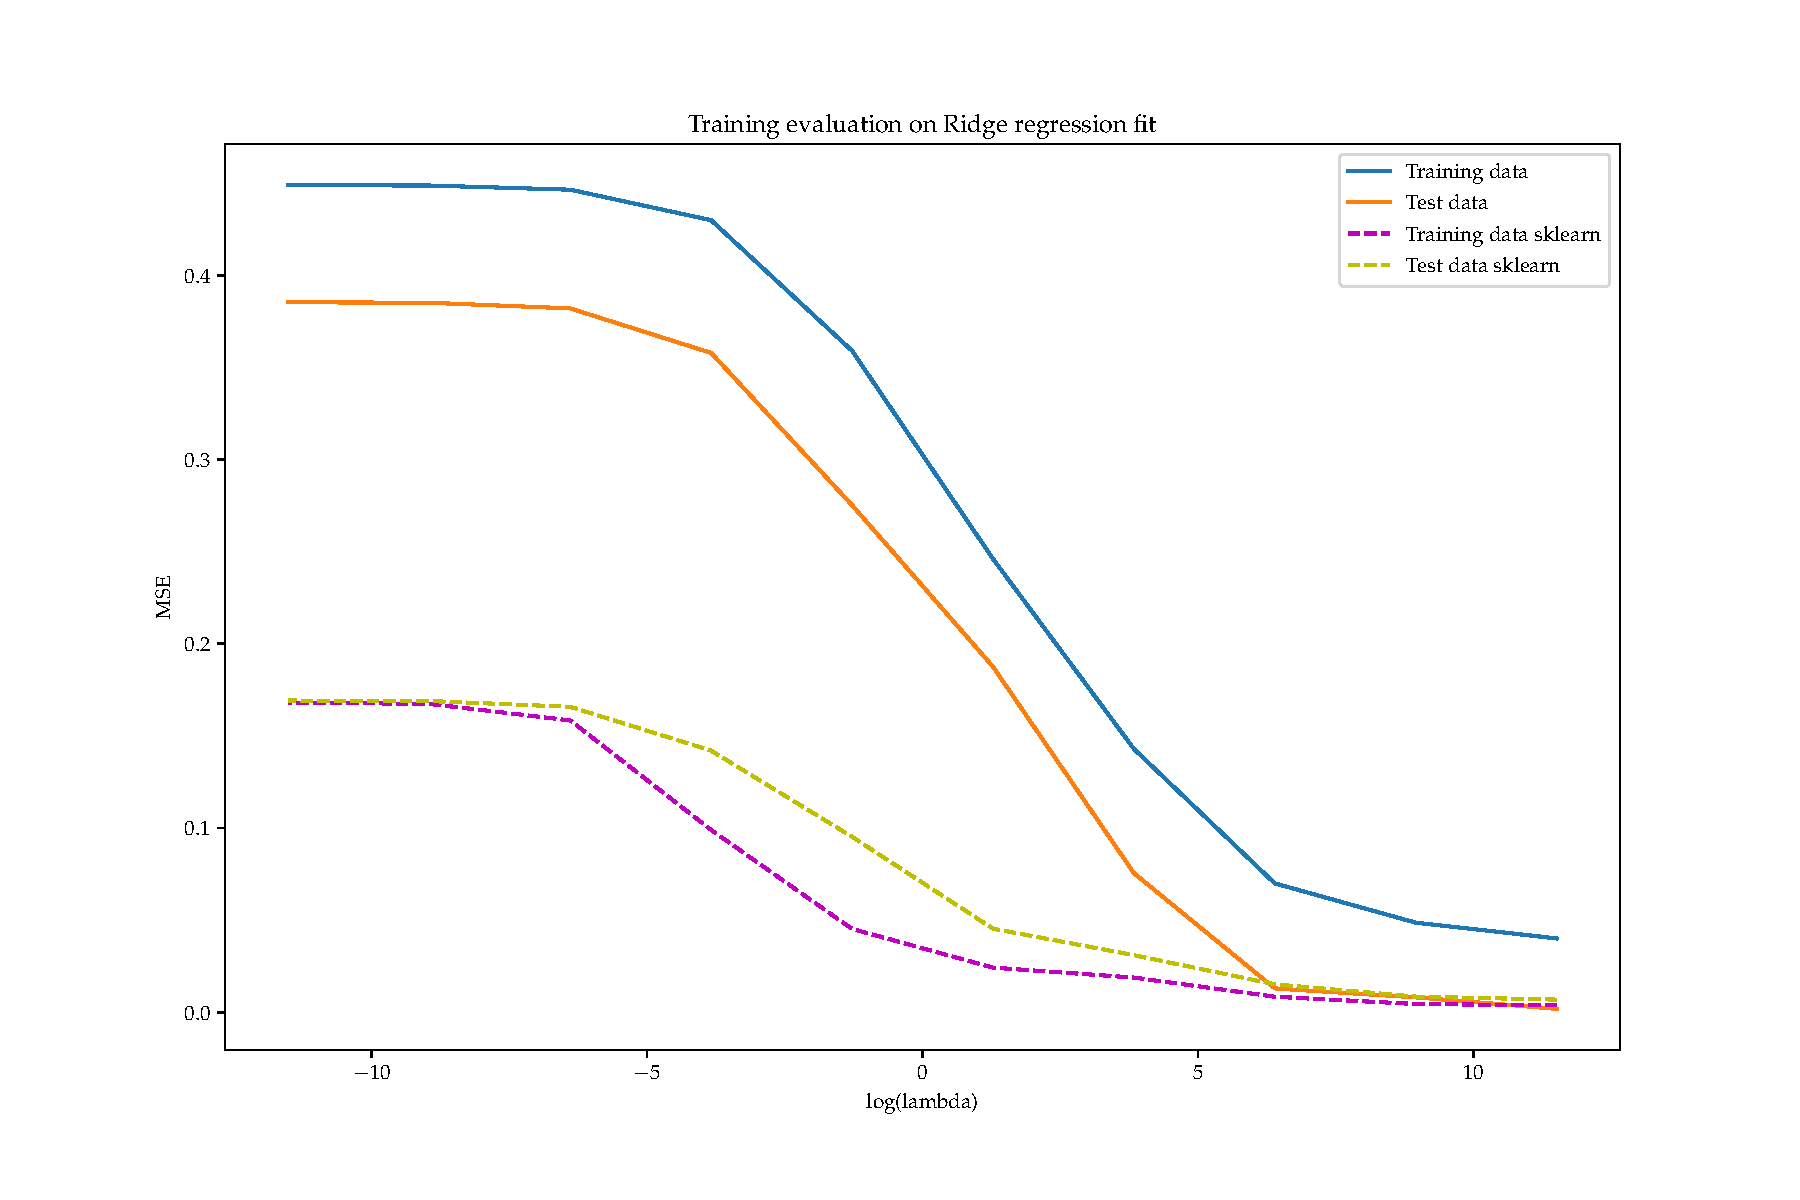
\includegraphics[scale=0.45]{figures/franke_function_Ridge_evaluate_fit.pdf}
  \caption{The best fit using Ridge}
  \label{fig: Ridge_best_fit}
\end{figure}

\begin{figure}
  \centering
  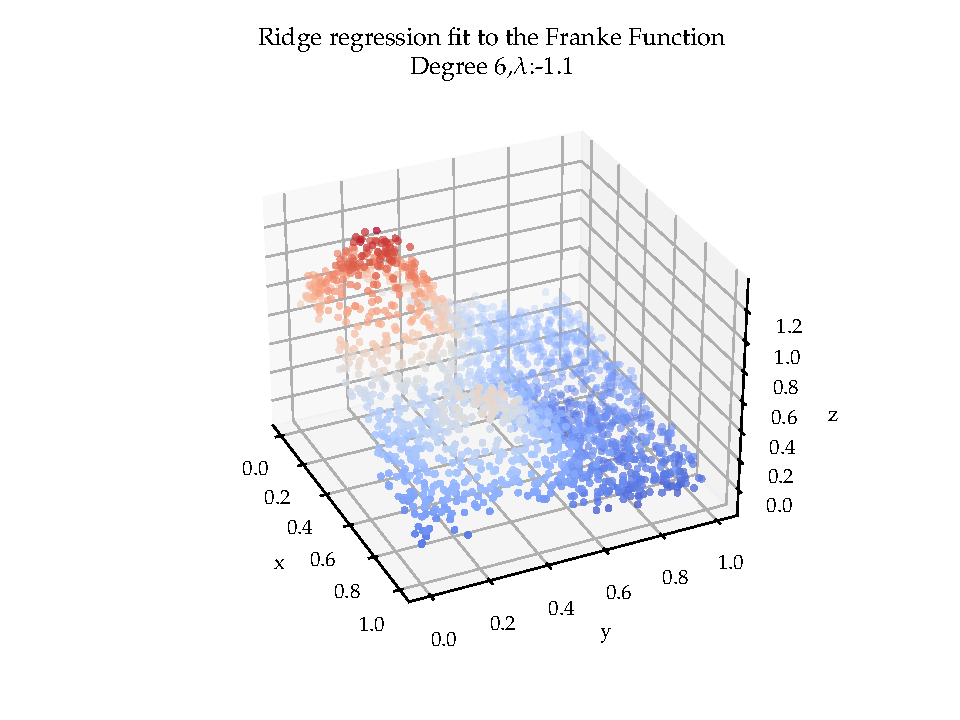
\includegraphics[scale=0.85]{figures/franke_function_Ridge_best_fit.pdf}
  \caption{The best fit using Ridge}
  \label{fig: Ridge_best_fit}
\end{figure}

\begin{center}
  \csvautobooktabular{data/report_data/redge_reg_lambda_-1.1.csv}
  \label{data: Ridge_best_fit}
\end{center}



\newpage
\newpage


\bibliography{bibliography}
\bibliographystyle{ieeetr}



\end{document}


% Local Variables:
% TeX-engine: xetex
% End:
